\documentclass[conference]{IEEEtran}
\IEEEoverridecommandlockouts
% The preceding line is only needed to identify funding in the first footnote. If that is unneeded, please comment it out.
\usepackage{cite}
\usepackage{amsmath,amssymb,amsfonts}
%\usepackage{algorithmic}
\usepackage{graphicx}
\usepackage{textcomp}
\usepackage{xcolor}
\usepackage{subcaption}
\usepackage{float} % H image float mode
\usepackage{hyperref}



\def\BibTeX{{\rm B\kern-.05em{\sc i\kern-.025em b}\kern-.08em
    T\kern-.1667em\lower.7ex\hbox{E}\kern-.125emX}}

%%%%%%%%%%%%%%%%%%%%%%%%%%%%%%%%%%%%%%%%%%%%%%%%%%%%%%%%%%%%%%%%%%%%%%%%%%%%%%%%%%%%%%%

\newenvironment{note}{
	\color{gray}
}

%%%%%%%%%%%%%%%%%%%%%%%%%%%%%%%%%%%%%%%%%%%%%%%%%%%%%%%%%%%%%%%%%%%%%%%%%%%%%%%%%%%%%%%

\hypersetup{
	colorlinks=true,
	linkcolor=blue,
	filecolor=magenta,      
	urlcolor=cyan,      
	citecolor=green,
	pdftitle={Métodos de Deep Learning aplicados à Segmentação Semântica de Imagens para Percepção de Veículos Autônomos}
}

\begin{document}

\title{\huge{Métodos de \textit{Deep Learning} aplicados à Segmentação Semântica de Imagens para Percepção de Veículos Autônomos}}

\author{\IEEEauthorblockN{Gabriel Toffanetto França da Rocha}
\IEEEauthorblockA{\textit{Laboratório de Mobilidade Autônoma -- LMA} \\
\textit{Faculdade de Engenharia Mecânica, Universidade Estadual de Campinas}}\\
Campinas, Brasil \\
g289320@dac.unicamp.br}

\maketitle

\begin{abstract}

%\begin{note}
%	\begin{itemize}
%		\item Veículos autonomos
%		\item Visão computacional
%		\item Percepção do ambiente
%		\item Segmentação Semântica de Imagem
%		\item Métodos Vanilla
%		\item Métodos Deep Learning
%		\item Necessidades da aplicação
%		\item Resultados
%		\item Proximos passos (teste para obtenção do Perception grid)
%	\end{itemize}
%\end{note}

\end{abstract}

\begin{IEEEkeywords}
Deep learning, Visão computacional, Segmentação Semântica de Imagem, Robótica móvel, Veículos autônomos
\end{IEEEkeywords}

\section{Introdução} \label{sc:introducao}

%% ToDo

%\begin{note}
%	
%	\begin{itemize}
%		\item Veículos autônomos 
%		\begin{itemize}
%			\item VILMA \cite{garcia2018VILMAIntelligentVehicle}
%		\end{itemize}
%		\item Métodos de navegação 
%		\begin{itemize}
%			\item Segmentação de imagem para mapeamento de área navegável e obstáculos \cite{jebamikyousAutonomousVehiclesPerception2022}
%			\item Citar método do Giovani \cite{vitor2021ModelingEvidentialGrids}
%		\end{itemize}
%		\item Comparar como era feito e como é feito hoje em dia
%		\item Mostrar a ideia vantajosa de utilizar \textit{Deep Learning}  \cite{geron2020HandsonMachineLearning}
%		\begin{itemize}
%			\item Dispensa de pré-processamento
%			\item Robustez à variação de luz, reflexos (desde que esses sejam usados em treinamento) \cite{papadeas2021RealTimeSemanticImage}
%			\item \textit{Datasets} para treinamento \cite{cordts2016CityscapesDatasetSemantic, brostow2008SegmentationRecognitionUsing, brostow2009SemanticObjectClasses, jin2021RaidaRRichAnnotated}
%		\end{itemize}
%	\end{itemize}
%
%
%\end{note}

Veículos com capacidade de se guiarem de forma autônoma estão cada vez mais presentes no dia a dia da sociedade contemporânea, possibilitando que o motorista possa realizar outras atividades durante a navegação, ou que o mesmo seja assistido em caso de alguma falha humana do condutor. Para que o automóvel seja capaz de se mover por conta própria, o mesmo deve ser capaz de perceber o ambiente, e sensores como sonares, radares, LiDARs e câmeras podem ser utilizados para tal. Porém, a câmera se faz como uma solução mais viável economicamente, e como visto na literatura, apresenta soluções que contemplam os desafios da navegação autônoma de veículos em ambientes urbanos, como visto nos trabalhos de \cite{garcia2018VILMAIntelligentVehicle} e \cite{vitor2014UrbanEnvironmentNavigation}.

Para que um veículo autônomo possa entender o ambiente à sua volta, é necessário que ele saiba reconhecer as entidades que o compõem, como por exemplo: estrada, veículos, calçadas, pedestres e vegetação, para que assim, o mesmo saiba diferenciar área navegável de obstáculos \cite{jebamikyousAutonomousVehiclesPerception2022}. Para isso, o emprego da técnica de segmentação semântica de imagens, onde cada pixel da imagem é classificado de acordo com a entidade do ambiente da qual ele faz parte \cite{he2016ImageSegmentationTechniques}. A Fig.~\ref{fig:dynamiclocalperception} mostra a aplicação da técnica de segmentação semântica fundida à informação de profundidade dada por uma câmera \textit{stereo}, permitindo a obtenção de um \textit{grid} de percepção dinâmica local (DLP), que projeta no plano 2D o ambiente contendo a detecção de múltiplos objetos para que o veículo consiga planejar seu caminho \cite{vitor2021ModelingEvidentialGrids}.

\begin{figure}[h!]
	\centering
	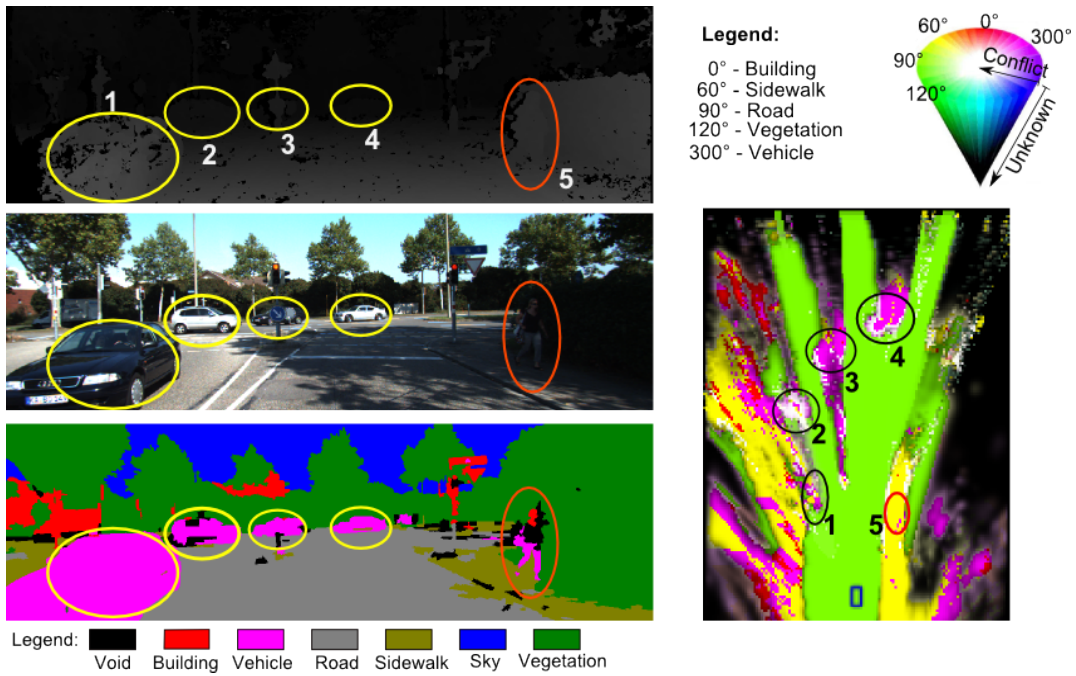
\includegraphics[width=\linewidth]{img/dynamic_local_perception}
	\caption{DLP com ênfase na detecção múltipla de objetos móveis obtido com a fusão da imagem semanticamente segmentada e as informações de profundidade \cite{vitor2021ModelingEvidentialGrids}.}
	\label{fig:dynamiclocalperception}
\end{figure}

Existem métodos de processamento de imagens que realizam o mascaramento de cada entidade da imagem, porém a definição de qual é a classe de cada segmento se faz desafiadora, sendo anteriormente empregada a utilização de redes neurais artificiais (ANNs) para tal, como feito por \cite{vitor20132D3DVision}. Porém, devido à utilização de ANNs somente para a classificação final, era necessário muito pré-processamento para realização da segmentação semântica. Com o desenvolvimento das redes neurais profundas (DNNs), obteve-se métodos com poder suficiente para que, dada uma imagem bruta de entrada e uma imagem de referência (\textit{ground truth}) segmentada para comparação, a rede profunda consegue aprender como realizar a segmentação da imagem do ambiente urbano, como nas várias arquiteturas mostradas por \cite{papadeas2021RealTimeSemanticImage}. Com a popularização desses métodos, já existem diversos conjuntos de dados para treinamento das DNNs, como vistos em \cite{cordts2016CityscapesDatasetSemantic} e \cite{brostow2008SegmentationRecognitionUsing,brostow2009SemanticObjectClasses}. Existem também \textit{datasets} que trazem cenas ainda mais desafiadoras, como o \cite{jin2021RaidaRRichAnnotated} que apresenta imagens urbanas durante noites chuvosas.

Dessa forma, a percepção do ambiente por meio de visão computacional se faz indispensável para o desenvolvimento dos veículos autônomos, e com isso, os métodos de \textit{deep learning} se fazem uma grande ferramenta para conseguir-se reconhecer as entidades de uma cena urbana com robustez às variações de luz e reflexos, sendo assim uma solução a ser explorada. Além do desempenho da segmentação semântica, o tempo demandado para tal operação também é vital, uma vez que durante a navegação, todos os módulos operam em tempo real, e a quantidade de \textit{frames} segmentados por segundo é uma informação importante. Dessa forma, esse trabalho propõem a utilização de redes neurais profundas com diferentes arquiteturas para a segmentação semântica de imagens de cenas urbanas, utilizados \textit{datasets} da literatura e para testes finais, utilizando imagens reais adquiridas pelo autor. Com esse teste, espera-se poder julgar se o treinamento da rede neural com conjuntos de dados da literatura conseguem gerar máquinas que generalizam bem para localidades não vistas durante o treinamento.

Este trabalho é dividido em seis partes, onde na Seção~\ref{sc:introducao} é realizada a motivação e contextualização da pesquisa e na Seção~\ref{sc:estado-da-arte} é apresentado o estado da arte, discorrendo sobre as soluções utilizadas atualmente. Com isso, a Seção~\ref{sc:metodologia} apresenta a metodologia a ser utilizada neste trabalho, seguida dos resultados obtidos na Seção~\ref{sc:resultados} e sua análise na Seção~\ref{sc:analise}. Por fim, são apresentadas as conclusões na Seção~\ref{sc:conclusoes} e as referências utilizadas.

\section{Estado da arte} \label{sc:estado-da-arte}

%\begin{note}
%	\begin{itemize}
%		\item Estratégias para operação em real time
%		\begin{itemize}
%			\item Depthwise separable convolution
%		\end{itemize}
%		\item Artigos \textit{Survey} \cite{jeba...}
%		\item Tipos de redes utilizadas \cite{chao2019HarDNetLowMemory,fan2021RethinkingBiSeNetRealtime, wang2019ESNetEfficientSymmetric, yu2020BiSeNetV2Bilateral, yu2018BiSeNetBilateralSegmentation,poudel2018ContextNetExploringContext,badrinarayanan2016SegNetDeepConvolutional} 
%		\item Resultados estado-da-arte \cite{papadeas2021RealTimeSemanticImage}
%		\begin{itemize}
%			\item mIoU
%			\item FPS
%		\end{itemize}
%	\end{itemize}
%\end{note}

As aplicações de \textit{deep learning} para solução de problemas de segmentação semântica de imagem vem trazendo resultados de alta performance, a partir de dados brutos, ou seja, sem a necessidade de pré-processamento das informações capturadas pela câmera. Porém, para que seja possível a realização dessa tarefa em tempo real, a literatura propõem a utilização de aproximações que permitem a redução do tempo de inferência \cite{papadeas2021RealTimeSemanticImage}. Entre tais métodos, se propõem a utilização de \textit{Depthwise Separable Convolution}, \textit{channel shuffling}, utilização de \textit{decoders} enxutos, redução eficiente do tamanho dos \textit{feature maps} e \textit{two-branch network}. A última em especial, sendo utilizada no presente trabalho, permite que sejam utilizada uma arquitetura mais leve, onde um ramo será suficientemente profundo para obter as informações semânticas da entrada, enquanto o outro é raso para captar os detalhes espaciais, ou seja, um ramo define os segmentos da imagem, e o outro os classifica.

O \textit{survey} \cite{papadeas2021RealTimeSemanticImage} demonstra a comparação entre diversas arquiteturas de redes neurais, ponderando o desempenho das mesmas, por meio da métrica mIoU, e o tempo de inferência, expressado em \textit{frames per second} (FPS). Estão presentes na comparação, redes baseadas em \textit{encoder-decoder}, U-Net, DenseNet, SENet e \textit{two-branch network}, onde as que derivam a arquitetura da última, como a BiSeNet \cite{yu2018BiSeNetBilateralSegmentation}, BiSeNet V2 \cite{yu2020BiSeNetV2Bilateral} e STDC \cite{fan2021RethinkingBiSeNetRealtime} apresentam as maiores velocidades de inferência, alcançando os 250 FPS, enquanto SqueezeNet \cite{treml2016SpeedingSemanticSegmentation} obtém o maior mIoU, obtendo 84,3 \%.


\section{Metodologia} \label{sc:metodologia}

%\begin{note}
%	\begin{itemize}
%		\item Arquiteturas escolhidas 
%		\item Redes escolhidas
%		\item \textit{Datasets} escolhidos
%		\begin{itemize}
%			\item Proposta de utilizar dados coletados no \textit{campus}
%		\end{itemize}
%		\item Método de treinamento
%		\item Métricas utilizadas
%		\item \textit{Frameworks} utilizados
%		\item \textit{Hardware} utilizado
%		
%	\end{itemize}
%\end{note}

Para a solução do problema foi escolhida uma rede da família STDC, que conseguem realizar a segmentação semântica de imagens de forma rápida e com desempenho estado da arte. Tal arquitetura apresenta grande riqueza de recursos, empregando inspirações na BiSeNet, SENet, U-Net e utilizando mecanismos de atenção, além da utilização de uma função de custo secundária para potencializar a captação de detalhes pela rede. A rede STDC75-1 foi escolhida por apresentar a maior velocidade nos testes realizados pelos autores do \textit{survey} \cite{papadeas2021RealTimeSemanticImage}, com um desempenho de segmentação considerável, permitindo uma melhor \textit{performance} no \textit{hardware} disponível.

\subsection{Arquitetura}

A rede STDC1 \cite{fan2021RethinkingBiSeNetRealtime} é baseada na arquitetura de \textit{two-branch network}, onde existe uma bifurcação da rede em dois ramos, um ligado à extração de informações de contexto e o outro aplicado para obtenção de informações espaciais da entrada. A informação de contexto demanda de uma maior profundidade, implementando mecanismos de atenção em dois níveis para extração dos atributos necessários para a identificação das regiões da imagem, como mostrado na Fig.~\ref{fig:stdcseg-architecture}(a).

\begin{figure}[h!]
	\centering
	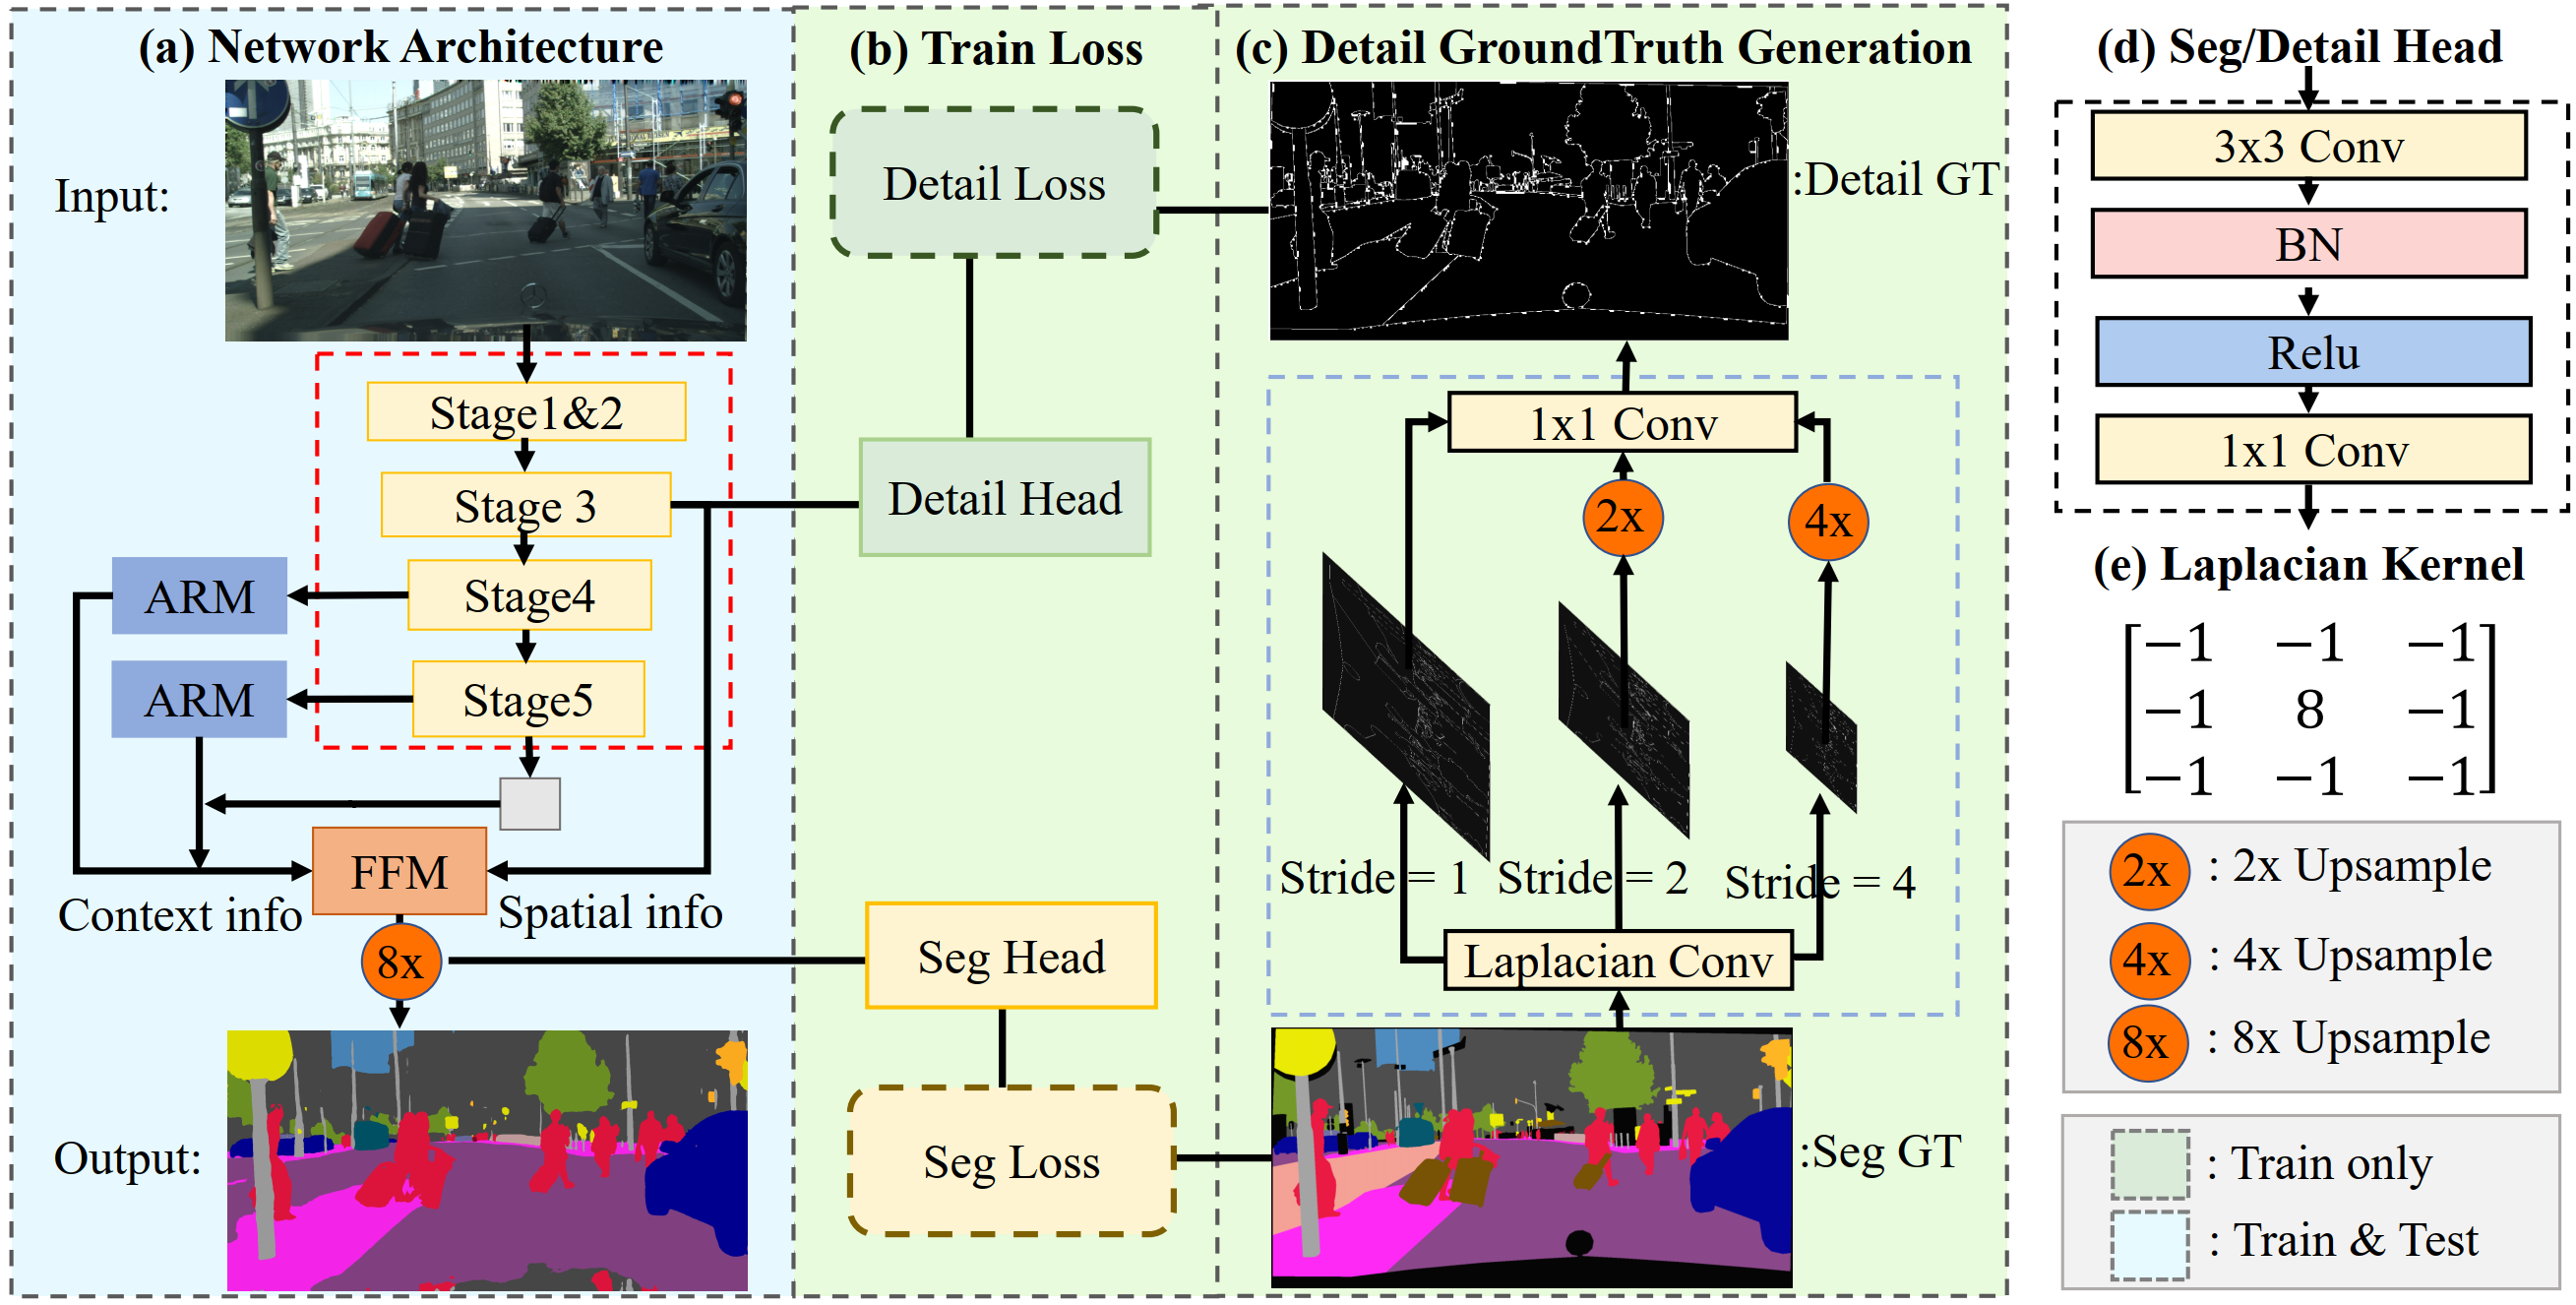
\includegraphics[width=1\linewidth]{img/stdcseg-architecture}
	\caption{Arquitetura completa da rede neural utilizada \cite{fan2021RethinkingBiSeNetRealtime}.}
	\label{fig:stdcseg-architecture}
\end{figure}

Porém, o fato de se processar a informação de entrada em dois ramos, traz um inconveniente para o problema de segmentação em tempo real, que é justamente o tempo de inferência da rede. Desta forma, a rede aplica uma estratégia elegante ao utilizar no lugar de um ramo com novas camadas, uma \textit{skip connection} do \textit{Stage 3}, para o bloco de fusão dos \textit{feature maps} oriundos dos dois braços da rede. Para forçar a captura das informações espaciais, a saída da \textit{skip connection} é utilizada em uma tarefa auxiliar de detecção de bordas de cada região semântica da imagem, por meio de uma \textit{detail head}, como visto na Fig.~\ref{fig:stdcseg-architecture}(b). Tal procedimento é realizado por meio de treinamento supervisionado, onde com a aplicação de filtros laplacianos na imagem rótulo de segmentação semântica, se obtém a imagem rótulo com as bordas de cada segmento da imagem de entrada, procedimento ilustrado na Fig.~\ref{fig:stdcseg-architecture}(c). Tal informação explicita os detalhes à serem capturados pelo ramo espacial, e a perda é computada por meio da saída da \textit{detail head} e o rótulo obtido. Reforça-se que esse procedimento é realizado apenas em treinamento, enquanto durante a inferência a rede neural irá utilizar as habilidades aprendidas por meio do gradiente sobre a perda atrelada à segmentação e à detecção de bordas, sem realizar explicitamente a extração das bordas de cada região da imagem.

O módulo principal da rede é o \textit{Short-Term Dense Concatenate Module} (STDC), que possuí quatro camadas internas de convolução (convolução + \textit{batch normalization} + ReLU), e os \textit{feature maps} de todas as camadas convolucionais do bloco são concatenadas na saída, formando assim um bloco com característica densa, como descrito na Fig. \ref{fig:stdc}. Dada uma entrada de $M$ canais, a primeira camada possuí \textit{kernels} $1 \times 1$, gerando $N/2$ \textit{feature maps}. A segunda camada realiza \textit{downsampling}, apresentando \textit{stride} = 2 e \textit{kernel} $3 \times 3$, assim como as consecutivas, porém contribuindo com $N/4$ canais de saída. Por fim, as duas ultimas camadas contribuem cada uma com $N/8$ mapas de ativação, e com isso, o bloco concatena todos os canais de saída, apresentando uma saída com $N$ canais. Tal configuração se fez para valorizar a tarefa de segmentação de imagem, onde nas primeiras camadas existem mais filtros, e com isso, conseguindo explorar melhor a extração de informação multi-escala \cite{fan2021RethinkingBiSeNetRealtime}.

\begin{figure}[h!]
	\centering
	\includegraphics[width=1\linewidth]{../../src/STDC-Seg/images/stdc}
	\caption{Estrutura do módulo STDC. Adaptado de \cite{fan2021RethinkingBiSeNetRealtime}.}
	\label{fig:stdc}
\end{figure}


O estágio 1 e 2 realizam a operação de convolução, \textit{batch normalization} e ReLU aos dados de entrada, com \textit{stride} igual a 2. Já os estágios 3, 4 e 5 apresentam realizações em série de módulo STDC. O mecanismo de atenção e o bloco \textit{Feature Fusion Module} (FFM) são baseados na rede BiSeNet \cite{yu2018BiSeNetBilateralSegmentation}, onde o funciona com base em obter os pesos de atenção por meio da aplicação de \textit{global pooling}, computando o vetor de pesos por uma camada convolucional com \textit{kernel} $1 \times 1$, aplicando \textit{batch normalization} e ativação logística. Dessa forma, a informação de contexto global é integrada com baixo custo computacional, evitando \textit{up-sampling}. Já o bloco FFM, é inspirado no conceito da SENet, e condiciona a soma as informações do ramo de contexto e do ramo espacial da rede \textit{two-branch}. O mesmo se faz por meio da concatenação dos \textit{feature maps}, normalização por \textit{batch normalization} e ponderação dessas informações por meio de um vetor de pesos obtido por meio da aplicação de \textit{global pooling}, e duas camadas de convolução de \textit{kernel} de tamanho unitário, a primeira seguida por ReLU e a segunda por uma sigmoide. Por fim é realizado um \textit{upsampling} de 8 vezes para a recuperação da dimensão de entrada.

Sua implementação se deu com base nos códigos fonte disponibilizados pelos autores da rede, modificados para o problema em questão, e disponibilizados no GitHub\footnote{\href{https://github.com/toffanetto/STDC-Seg}{github.com/toffanetto/STDC-Seg}}. Utilizou-se o \textit{framework} PyTorch, juntamente dos pacotes de CUDA necessários para utilização da GPU NVIDIA em treinamento e inferência.


\subsection{\textit{Dataset} de treinamento e dados de teste}

O conjunto de dados Cityscapes \cite{cordts2016CityscapesDatasetSemantic} foi escolhido como base para treinamento e avaliação do modelo, sendo um \textit{dataset} que contempla imagens de alta resolução, de contextos urbanos, capturados em diversas cidades da Europa. A base de dados conta com a anotação de 30 classes, sendo que 19 estão disponíveis para o problema de segmentação semântica, sendo elas: estrada, calçada, pedestre, piloto/condutor, carro, caminhão, ônibus, trem, moto, bicicleta, edifício, muro, cerca, poste, placa de transito, semáforo, vegetação, terreno e céu, cuja legenda está disponível na Fig.~\ref{fig:legend}. Estão disponíveis no mesmo, 5000 imagens com anotação fina dos segmentos semânticos, divididos em treinamento (2975), validação (500) e teste (1525). A resolução das imagens é de $2048 \times 1024$ pixels, sendo uma entrada desafiadora para a inferência em tempo real.

\begin{figure}[h!]
	\centering
	\includegraphics[width=1\linewidth]{../../src/STDC-Seg/output/legend.pdf}
	\caption{Legenda de cores referentes à cada classe do \textit{dataset}.}
	\label{fig:legend}
\end{figure}

Foram implementadas estratégias de \textit{data augmentation} pelos autores da rede neural \cite{fan2021RethinkingBiSeNetRealtime}, utilizando alteração de cor, brilho e contraste, inversão horizontal, aplicação de escala e corte, buscando a inserção de robustez e maximização da capacidade de generalização, evitando \textit{overfitting}. A aplicação de escala também é utilizada para reduzir a dimensão dos dados de entrada, facilitando a predição do mapa de segmentação semântico em tempo real pela rede, onde foi escolhida a escala de 0,75 por fornecer um desempenho maior.

Para teste da capacidade de generalização do modelo, realizou-se uma coleta de dados na mesma forma da realizada pelos autores do \textit{dataset}, no \textit{campus} da Unicamp, sendo assim, imagens de locais que não foram vistos em treinamento, e aplicou-se a inferência da máscara de segmentação semântica das mesmas por meio da rede STCD1.

\subsection{Método de treinamento}

%\textit{\color{gray}
%	\begin{itemize}
%		\item mini-batch SGD com momento e decaimento
%		\item poly learning rate policy
%		\item 60000 interações
%		\item Função de custo?
%\end{itemize}}

O treinamento da rede neural foi realizado por meio do algoritmo de gradiente descendente estocástico (SGD), com \textit{momentum} de 0,9, decaimento de pesos de $5e^{-4}$, com atualização dos pesos por \textit{mini-batch} de 4 amostras, devido às limitações de memória da GPU utilizada. O treinamento é limitado por número de iterações, onde com base na rede original, foi limitado em 60000 iterações, onde é adotada uma estratégia de \textit{warmup}. Com isso, a taxa de aprendizado é incrementada de um valor pequeno até o valor alvo durante as primeiras 1000 interações para estabilização do processo de otimização e evitar a divergência do mesmo. Além disso, durante o treinamento a taxa de aprendizado é adaptada por meio de uma política polinomial, dada por $(1 - iter/max\_iter)^{power}$, onde foi considerada uma potência de 0.9 \cite{fan2021RethinkingBiSeNetRealtime}.

Como função de custo para ajuste dos pesos, é considerada a entropia cruzada, por se tratar de um problema de classificação, e aplicando recursos \textit{Online Hard Example Mining} para a otimização da tarefa de aprendizado da segmentação semântica. O OHEM é uma estratégia de exploração de amostras desafiadoras, que tendem a trazer mais aprendizado ao modelo devido à riqueza de informações transpassadas pela complexidade de classificação, sendo selecionados durante o treinamento, e trazendo mais robustez à rede \cite{shrivastava2016TrainingRegionbasedObject}. 

Também é computada a função de custo para o problema de detecção dos detalhes, realizado pela \textit{detail head}. Nesse caso, não é utilizado a entropia cruzada, devido a ser um problema altamente desbalanceado, onde a mesma não apresenta bons resultado. Nesse caso, são aplicadas as métricas de entropia cruzada binária e \textit{dice loss}, conforme \eqref{eq:ldetail}. A \textit{dice loss}, enunciada em \eqref{eq:ldice} se baseia em medir a sobreposição entre o mapa predito e seu respectivo rótulo, variando no intervalo [0, 1], sendo assim robusta ao número de pixels de cada classe. O equacionamento é realizado considerando uma entrada de $H \times W$ pixels, obtendo assim uma predição do mapa de detalhes $p_d$, sendo $g_d$ seu respectivo rótulo, e $\epsilon$ uma constante para evitar a divisão por zero \cite{deng2018LearningPredictCrisp}.

\begin{gather}
	L_{detail}(p_d,g_d) = L_{dice}(p_d, g_d) + L_{bce}(p_d, g_d) \label{eq:ldetail} \\ 
	L_{dice}(p_d, g_d) = 1 - \frac{2\sum_{i}^{H\times W}p_d^ig_d^i + \epsilon}{\sum_{i}^{H\times W}(p_d^i)^2 + \sum_{i}^{H\times W}(g_d^i)^2 + \epsilon}
	\label{eq:ldice}
\end{gather}


\subsection{Métricas de avaliação}

Sendo um problema de segmentação com $k +1$ classes considerando o fundo da imagem, têm-se que $p_{ij}$ é o número de pixels pertencentes à classe $i$ que foram preditos para a classe $j$, logo, $i = j$ representa uma classificação correta da classe do pixel.

Com isso, as duas métricas mais famosas para segmentação semântica, sendo elas a \textit{Intersection over Union} (IoU) e \textit{mean Intersection over Union} (mIoU). A IoU, enunciada em \eqref{eq:IoU}, é obtida pela quantidade de pixels preditos corretamente para uma certa classe (interseção predição e \textit{ground truth}), divido pela quantidade de pixels preditos incorretamente somado ao \textit{ground truth} (união) \cite{papadeas2021RealTimeSemanticImage}. 

\begin{equation}\label{eq:IoU}
	\text{IoU} = \frac{\sum_{i=0}^{k}p_{ii}}{\sum_{i=0}^{k}\sum_{j=0}^{k}\left(p_{ij} + p_{ji}\right) - \sum_{i=0}^{k}p_{ii}}
\end{equation}

Ao realizar a média da IoU para $k+1$ classes, se obtém a mIoU, conforme \eqref{eq:mIoU}. Devido à informação de um desempenho médio para todas as classes, essa métrica foi escolhida para realização da medida de efetividade da segmentação semântica.

\begin{equation}\label{eq:mIoU}
	\text{mIoU} = \frac{1}{k+1} \sum_{i = 0}^{k}\frac{p_{ii}}{\sum_{j=0}^{k}\left(p_{ij} + p_{ji}\right) - p_{ii}}
\end{equation}



\section{Resultados}  \label{sc:resultados}

%\begin{note}
%	\begin{itemize}
%		\item Para cada rede:
%		\begin{itemize}
%			\item Métricas 
%			\item Segmentação
%			\begin{itemize}
%				\item Entrada
%				\item \textit{Ground truth}
%				\item Saída
%			\end{itemize}
%			\item Tempo de treinamento
%		\end{itemize}
%	\end{itemize}
%\end{note}

\subsection{Métricas de teste}

Ao realizar a validação da rede treinada para as 500 amostras de teste do conjunto de validação do \textit{dataset} Cityscapes, obteve-se um índice de mIOU igual a \textbf{74,5046\%}.

\subsection{Cityscapes}

\begin{figure}[h!]
	
\begin{subfigure}[H]{\linewidth}
\centering
\includegraphics[width=1\linewidth]{../../src/STDC-Seg/output/sample_frankfurt_000001_077434}
\caption{}
\label{fig:sample_munster_000036_000019}
\end{subfigure}

\begin{subfigure}[H]{\linewidth}
\centering
\includegraphics[width=1\linewidth]{../../src/STDC-Seg/output/sample_munster_000078_000019}
\caption{}
\label{fig:sample_munster_000078_000019}
\end{subfigure}

\begin{subfigure}[H]{\linewidth}
\centering
\includegraphics[width=1\linewidth]{../../src/STDC-Seg/output/sample_frankfurt_000001_046272}
\caption{}
\label{fig:sample_frankfurt_000001_046272}
\end{subfigure}

\begin{subfigure}[H]{\linewidth}
	\centering
	\includegraphics[width=1\linewidth]{../../src/STDC-Seg/output/sample_frankfurt_000001_059119}
	\caption{}
	\label{fig:sample_frankfurt_000001_059119}
\end{subfigure}
\caption{Predições para cenas do \textit{dataset} Cityscapes.}
\label{fig:result_cityscapes}
\end{figure}


\subsection{Unicamp}


\section{Análise dos Resultados}  \label{sc:analise}

%\begin{note}
%	\begin{itemize}
%		\item Comparar as três redes:
%		\begin{itemize}
%			\item mIoU
%			\item FPS
%			\item Dados segmentados do \textit{dataset}
%			\item Dados segmentados coletados no \textit{campus}
%		\end{itemize}
%		\item Apontar relação custo \textit{vs} desempenho de cada rede
%		\item Considerar custos de treinamento
%	\end{itemize}
%\end{note}

A partir do resultado de mIoU obtido, pode-se dizer que a rede treinada obtida está entre as concorrentes do estado da arte. Analisando algumas amostras tomadas do dados de teste, observa-se na Fig. \ref{fig:result_cityscapes}(\subref{fig:sample_munster_000036_000019}) a detecção precisa do ciclista, dos pedestres, e também a diferenciação entre a rua e a calçada, que visualmente não apresentam grande diferença. Já na Fig. \ref{fig:result_cityscapes}(\subref{fig:sample_munster_000078_000019}), é possível ver a definição das entidades do trânsito, como carros, caminhões, semáforos e placas, assim como seus respectivos postes. Novamente, a ciclovia é reconhecida como calçada. Por fim, as imagens das Fig. \ref{fig:result_cityscapes}(\subref{fig:sample_frankfurt_000001_046272})~e~\ref{fig:result_cityscapes}(\subref{fig:sample_frankfurt_000001_059119}) se mostram mais desafiadores, uma vez que possuem sombras. Porém, a rede neural consegue com facilidade definir a rua, os pedestres, a calçada e as placas de sinalização mesmo com a presença de diferentes níveis de iluminação da cena.

\section{Conclusões}  \label{sc:conclusoes}

%\begin{note}
%	\begin{itemize}
%		\item Retomar o problema inicial
%		\item Destacar metodologia e os resultados que foram obtidos
%		\item Comentar a análise dos resultados, mostrando que seria melhor para implementação
%		\item Propor melhorias
%		\item Propor validação de aplicação
%		\item Listar proposta de aplicação dessa técnica
%		\begin{itemize}
%			\item Perception grid
%		\end{itemize}
%	\end{itemize}
%\end{note}

\section*{Agradecimentos}

%\begin{note}
%	\begin{itemize}
%		\item Levy e Romis
%	\end{itemize}
%\end{note}

Deixo meus agradecimentos aos professores Dr. Levy Boccato e Dr. Romis Attux, por todos os conhecimentos compartilhados e que tornaram possível a realização deste trabalho.

\section*{Referências}  \label{sc:referencias}

\nocite{geron2020HandsonMachineLearning}

\bibliographystyle{acm}
\renewcommand{\section}[2]{}
\bibliography{bibliograpy}

\end{document}